\documentclass[tikz,margin=1mm]{standalone}
\usepackage{xcolor,amsmath}

 \usetikzlibrary{arrows.meta,chains, decorations.pathreplacing,bending,positioning}



\begin{document}
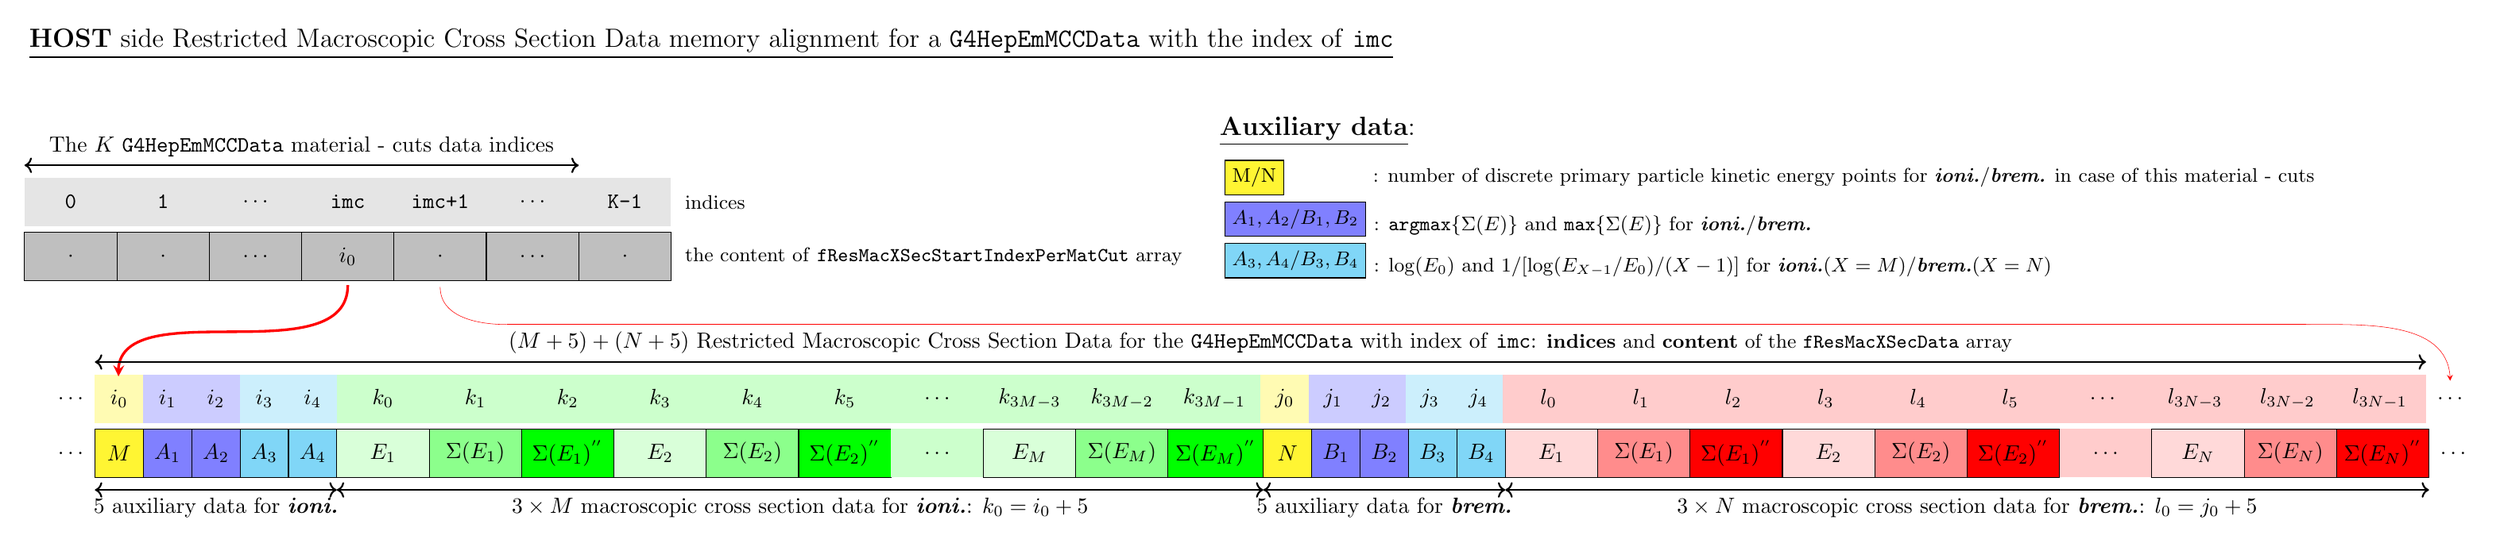
\begin{tikzpicture}[
   start chain       = going right,
   node distance = 0pt,
    %
   noStyle/.style  = {draw=none, minimum width=2.2em, minimum height=2.2em, outer sep=0pt, font=\ttfamily, on chain},
   %
   eiStyle1/.style  = {draw=none, minimum width=2.2em, minimum height=2.2em, outer sep=0pt, font=\ttfamily, on chain, fill=yellow!30},
   eStyle1/.style   = {draw, minimum width=2.2em, minimum height=2.2em, outer sep=0pt, on chain, fill=yellow!80},
   eiStyle2/.style  = {draw=none, minimum width=2.2em, minimum height=2.2em, outer sep=0pt, font=\ttfamily, on chain, fill=blue!20},
   eStyle2/.style   = {draw, minimum width=2.2em, minimum height=2.2em, outer sep=0pt, on chain, fill=blue!50},
   eiStyle3/.style  = {draw=none, minimum width=2.2em, minimum height=2.2em, outer sep=0pt, font=\ttfamily, on chain, fill=cyan!20},
   eStyle3/.style   = {draw, minimum width=2.2em, minimum height=2.2em, outer sep=0pt, on chain, fill=cyan!50},
   %
   imcStyle/.style      = {draw=none, minimum width=4.2em, minimum height=2.2em, outer sep=0pt, font=\ttfamily, on chain, fill=gray!20},
   mcStyle/.style     = {draw, minimum width=4.2em, minimum height=2.2em, outer sep=0pt, font=\ttfamily, on chain, fill=gray!50},
   %
   iIoniStyle/.style      = {draw=none, minimum width=4.2em, minimum height=2.2em, outer sep=0pt, font=\ttfamily, on chain, fill=green!20},
   ioniEStyle/.style     = {draw, minimum width=4.2em, minimum height=2.2em, outer sep=0pt, font=\ttfamily, on chain, fill=green!15},
   ioniSStyle/.style      = {draw, minimum width=4.2em, minimum height=2.2em, outer sep=0pt, font=\ttfamily, on chain, fill=green!45},
   ioniSDStyle/.style   = {draw, minimum width=4.2em, minimum height=2.2em, outer sep=0pt, font=\ttfamily, on chain, fill=green},
   %
   %
   iBremStyle/.style      = {draw=none, minimum width=4.2em, minimum height=2.2em, outer sep=0pt, font=\ttfamily, on chain, fill=red!20},
   bremEStyle/.style     = {draw, minimum width=4.2em, minimum height=2.2em, outer sep=0pt, font=\ttfamily, on chain, fill=red!15},
   bremSStyle/.style      = {draw, minimum width=4.2em, minimum height=2.2em, outer sep=0pt, font=\ttfamily, on chain, fill=red!45},
   bremSDStyle/.style   = {draw, minimum width=4.2em, minimum height=2.2em, outer sep=0pt, font=\ttfamily, on chain, fill=red},
  ]

    \begin{scope}[start chain=IMCINDX going right];
        \node [imcStyle] (IMC1) {$\texttt{0}$};
        \node [imcStyle] (IMC2) {$\texttt{1}$};
        \node [imcStyle] (IMC3) {$\ldots$};
        \node [imcStyle] (IMC4) {$\texttt{imc}$};
        \node [imcStyle] (IMC4p) {$\texttt{imc+1}$};
        \node [imcStyle] (IMC5) {$\ldots$};
        \node [imcStyle] (IMC6) {$\texttt{K-1}$};
    \end{scope}
   \draw[<->, thick] ([yshift=+2mm]IMCINDX-1.north west) -- node[above] {The $K$ \texttt{G4HepEmMCCData} material - cuts data indices} ([yshift=+2mm]IMCINDX-6.north east);

    \begin{scope}[start chain=MCINDX going right];
       \node [mcStyle, anchor=north, at={([yshift=-1mm]IMCINDX-1.south)}] (MC1) {$\cdot$};
       \node [mcStyle] (MC2) {$\cdot$};
        \node [mcStyle] (MC3) {$\ldots$};
        \node [mcStyle] (MC4) {$i_0$};
         \node [mcStyle] (MC4p) {$\cdot$};
        \node [mcStyle] (MC5) {$\ldots$};
        \node [mcStyle] (MC6) {$\cdot$};
    \end{scope}

    \node[anchor=north, at={([yshift=+25mm,xshift=+95mm]IMCINDX-1.north east)}] {\large {\underline{\textbf{HOST} side Restricted Macroscopic Cross Section Data memory alignment  for a \texttt{G4HepEmMCCData}  with the index of \texttt{imc}} }};

 \node[anchor=west, at={([yshift=0mm,xshift=1mm]IMCINDX-7.east)}] {\small {indices}};
 \node[anchor=west, at={([yshift=0mm,xshift=1mm]MCINDX-7.east)}] {\small {the content of \texttt{fResMacXSecStartIndexPerMatCut} array}};



    \begin{scope}[start chain=IDATA going right];
        \node [noStyle, anchor=north, at={([yshift=-15mm]MCINDX-1.south)}]  (id0) {$\ldots$};
        \node [eiStyle1] (id1) {$i_0$};
        \node [eiStyle2] (id2) {$i_1$};
        \node [eiStyle2] (id3) {$i_2$};
        \node [eiStyle3] (id4) {$i_3$};
        \node [eiStyle3] (id5) {$i_4$};
        \node [iIoniStyle] (id6) {$k_0$};
        \node [iIoniStyle] (id7) {$k_1$};
        \node [iIoniStyle] (id8) {$k_2$};
        \node [iIoniStyle] (id9) {$k_3$};
        \node [iIoniStyle] (id10) {$k_4$};
        \node [iIoniStyle] (id11) {$k_{5}$};
        \node [iIoniStyle] (id12) {$\ldots$};
        \node [iIoniStyle] (id13) {$k_{3M-3}$};
        \node [iIoniStyle] (id14) {$k_{3M-2}$};
        \node [iIoniStyle] (id15) {$k_{3M-1}$};
%        
        \node [eiStyle1] (id1) {$j_0$};
        \node [eiStyle2] (id2) {$j_1$};
        \node [eiStyle2] (id3) {$j_2$};
        \node [eiStyle3] (id4) {$j_3$};
        \node [eiStyle3] (id5) {$j_4$};
        \node [iBremStyle] (id6) {$l_0$};
        \node [iBremStyle] (id7) {$l_1$};
        \node [iBremStyle] (id8) {$l_2$};
        \node [iBremStyle] (id9) {$l_3$};
        \node [iBremStyle] (id10) {$l_4$};
        \node [iBremStyle] (id11) {$l_{5}$};
        \node [iBremStyle] (id12) {$\ldots$};
        \node [iBremStyle] (id13) {$l_{3N-3}$};
        \node [iBremStyle] (id14) {$l_{3N-2}$};
        \node [iBremStyle] (id15) {$l_{3N-1}$};
        \node [noStyle] (id16) {$\ldots$};
    \end{scope}

    \path[>=stealth, very thick,  shorten <=2pt,  shorten >=2pt, red] (MCINDX-4.south)  edge[in=100, out=-90, ->]  ([yshift=-1mm,xshift=0mm]IDATA-2.north);
    \path[>=stealth, very thin, red] ([yshift=-1mm]MCINDX-5.south)  edge[in=180, out=-90]  ([yshift=+8mm,xshift=5mm]IDATA-8.north)
         ([yshift=+8mm,xshift=5mm]IDATA-8.north) edge[] ([yshift=+8mm,xshift=3mm]IDATA-30.north)
         ([yshift=+8mm,xshift=3mm]IDATA-30.north)  edge[in=90, out=0, ->] ([yshift=-1mm,xshift=0mm]IDATA-32.north);

    \begin{scope}[start chain=DATA going right];
       \node [noStyle, anchor=north, at={([yshift=-1mm]IDATA-1.south)}] (d0) {$\ldots$};
        \node [eStyle1] (id1) {$M$};
        \node [eStyle2] (id2) {$A_1$};
        \node [eStyle2] (id3) {$A_2$};
        \node [eStyle3] (id4) {$A_3$};
        \node [eStyle3] (id5) {$A_4$};
        \node [ioniEStyle] (id6) {$E_1$};
        \node [ioniSStyle] (id7) {$\Sigma(E_1)$};
        \node [ioniSDStyle] (id8) {$\Sigma(E_1)^{''}$};
        \node [ioniEStyle] (id9) {$E_2$};
        \node [ioniSStyle] (id10) {$\Sigma(E_2)$};
        \node [ioniSDStyle] (id11) {$\Sigma(E_2)^{''}$};
        \node [iIoniStyle] (id12) {$\ldots$};
        \node [ioniEStyle] (id13) {$E_M$};
        \node [ioniSStyle] (id14) {$\Sigma(E_M)$};
        \node [ioniSDStyle] (id15) {$\Sigma(E_M)^{''}$};
%
        \node [eStyle1] (id1) {$N$};
        \node [eStyle2] (id2) {$B_1$};
        \node [eStyle2] (id3) {$B_2$};
        \node [eStyle3] (id4) {$B_3$};
        \node [eStyle3] (id5) {$B_4$};
        \node [bremEStyle] (id6) {$E_1$};
        \node [bremSStyle] (id7) {$\Sigma(E_1)$};
        \node [bremSDStyle] (id8) {$\Sigma(E_1)^{''}$};
        \node [bremEStyle] (id9) {$E_2$};
        \node [bremSStyle] (id10) {$\Sigma(E_2)$};
        \node [bremSDStyle] (id11) {$\Sigma(E_2)^{''}$};
        \node [iBremStyle] (id12) {$\ldots$};
        \node [bremEStyle] (id13) {$E_N$};
        \node [bremSStyle] (id14) {$\Sigma(E_N)$};
        \node [bremSDStyle] (id15) {$\Sigma(E_N)^{''}$};
        \node [noStyle] (id16) {$\ldots$};
    \end{scope}

     
      \draw[<->, thick] ([yshift=+2mm]IDATA-2.north west) -- node[above] {$(M+5)+(N+5)$ Restricted Macroscopic Cross Section Data for the \texttt{G4HepEmMCCData} with index of \texttt{imc}: \small {\textbf{indices} and \textbf{content} of the \texttt{fResMacXSecData} array}} ([yshift=+2mm]IDATA-31.north east);


      \draw[<->, thick] ([yshift=-2mm]DATA-2.south west) -- node[below] {$5$ auxiliary data for \textbf{\textit{ioni.}}} ([yshift=-2mm]DATA-6.south east);
      \draw[<->, thick] ([yshift=-2mm]DATA-7.south west) -- node[below] {$3\times M$ macroscopic cross section data for \textbf{\textit{ioni.}}: $k_0=i_0+5$} ([yshift=-2mm]DATA-16.south east);
      \draw[<->, thick] ([yshift=-2mm]DATA-17.south west) -- node[below] {$5$ auxiliary data for \textbf{\textit{brem.}}} ([yshift=-2mm]DATA-21.south east);
      \draw[<->, thick] ([yshift=-2mm]DATA-22.south west) -- node[below] {$3\times N$ macroscopic cross section data for \textbf{\textit{brem.}}: $l_0=j_0+5$} ([yshift=-2mm]DATA-31.south east);



     \node[anchor=west, at={([yshift=+20mm,xshift=175mm]MCINDX-1.east)}] (AUXData) {\large \underline{\textbf{Auxiliary data}}:};
     \node[anchor=north west, fill=yellow!80, draw=black, at={([yshift=-1mm,xshift=2mm]AUXData.south west)}] (au0) {\small {M/N}};
     \node[anchor=west, at={([xshift=13mm]au0.east)}] {\small {: number of discrete primary particle kinetic energy points for \textit{\textbf{ioni.}}/\textit{\textbf{brem.}} in case of this material - cuts}};
     \node[anchor=north west, fill=blue!50, draw=black, at={([yshift=-1mm]au0.south west)}] (au1) {\small {$A_1,A_2/B_1,B_2$}};
     \node[anchor=west, at={([yshift=-1mm]au1.east)}] {\small {: \texttt{argmax}$\{\Sigma(E)\}$ and \texttt{max}$\{\Sigma(E)\}$ for \textit{\textbf{ioni.}}/\textit{\textbf{brem.}} }};
     \node[anchor=north west, fill=cyan!50, draw=black, at={([yshift=-1mm]au1.south west)}] (au2) {\small {$A_3,A_4/B_3,B_4$}};
     \node[anchor=west, at={([yshift=-1mm]au2.east)}] {\small {: $\log(E_0)$ and $1/[\log(E_{X-1}/E_0)/(X-1)]$ for \textit{\textbf{ioni.}}($X=M$)/\textit{\textbf{brem.}}($X=N$) }};


\end{tikzpicture}
\end{document}
